% ============================================================
%  Nội dung báo cáo — chèn vào template LaTeX của nhóm
%  Biên dịch với: pdflatex hoặc xelatex (cần gói inputenc/fontenc hoặc fontspec)
% ============================================================

% ---- Preamble tối giản (bỏ nếu đã có template) ------------
\documentclass[12pt,a4paper]{article}
\usepackage[utf8]{inputenc}
\usepackage[T5]{fontenc}
\usepackage[vietnamese]{babel}
\usepackage{geometry}
\geometry{margin=2.5cm}
\usepackage{graphicx}
\usepackage{listings}
\usepackage{xcolor}
\usepackage{hyperref}
\usepackage{booktabs}
\usepackage{longtable}
\usepackage{array}
\usepackage{float}        % [H] — pin float exactly here
\usepackage{caption}
\usepackage{subcaption}


\lstset{
    basicstyle=\ttfamily\small,
    breaklines=true,
    frame=single,
    backgroundcolor=\color{gray!10},
    keywordstyle=\color{blue},
    commentstyle=\color{green!60!black},
    stringstyle=\color{red!70!black},
    numbers=left,
    numberstyle=\tiny\color{gray},
}

\title{\textbf{Báo Cáo Dự Án: YoloUNO PlatformIO-RTOS}\\
       \large Môn học: Internet of Things}
\author{Nhóm sinh viên}
\date{22/05/2026}
% ---- Kết thúc preamble tối giản ----------------------------

\begin{document}
\maketitle
\tableofcontents
\newpage

% ============================================================
\section{Giới Thiệu}
% ============================================================

Dự án xây dựng một hệ thống IoT nhúng toàn diện trên bo mạch \textbf{YOLO UNO} (chip ESP32-S3 Dual Core 240~MHz, 4~MB Flash, 8~MB PSRAM) sử dụng framework Arduino trên PlatformIO kết hợp với \textbf{FreeRTOS} để quản lý đa nhiệm theo thời gian thực.

Hệ thống thu thập dữ liệu từ cảm biến nhiệt độ/độ ẩm DHT20, xử lý và phân phối qua các cơ chế RTOS (Queue và Semaphore), điều khiển LED, NeoPixel, LCD, đồng thời cung cấp giao diện web, chạy mô hình TinyML phát hiện bất thường và đẩy dữ liệu lên nền tảng đám mây CoreIOT.

Những điểm nổi bật của hệ thống:
\begin{itemize}
    \item \textbf{Đa nhiệm theo thời gian thực:} 8 FreeRTOS Task chạy song song, mỗi task đảm nhận một chức năng độc lập.
    \item \textbf{Truyền dữ liệu an toàn:} Dữ liệu cảm biến truyền hoàn toàn qua Queue và Semaphore — không sử dụng biến toàn cục.
    \item \textbf{Giao diện web thời gian thực:} Dashboard 4 trang với WebSocket, đồng hồ gauge và điều khiển relay động.
    \item \textbf{TinyML trên vi điều khiển:} Mô hình ANN 33 tham số (1928 bytes) chạy trực tiếp trên ESP32-S3 để phát hiện bất thường môi trường.
    \item \textbf{Kết nối đám mây:} Đẩy telemetry lên CoreIOT qua giao thức MQTT theo chuẩn ThingsBoard.
\end{itemize}

\subsection{Mục Tiêu Cụ Thể}

\begin{table}[H]
\centering
\begin{tabular}{|c|p{11cm}|}
\hline
\textbf{Task} & \textbf{Nhiệm vụ} \\
\hline
Task 1 & LED đơn chớp theo ít nhất 3 điều kiện nhiệt độ; dùng semaphore đồng bộ \\
Task 2 & Điều khiển NeoPixel với ít nhất 3 mức màu theo độ ẩm; dùng semaphore \\
Task 3 & Giám sát T/H hiển thị LCD với ít nhất 3 trạng thái; loại bỏ biến toàn cục \\
Task 4 & Web server chế độ AP; giao diện điều khiển ít nhất 2 thiết bị, 2 nút \\
Task 5 & Triển khai TinyML trên vi điều khiển; mô tả dataset; đánh giá độ chính xác \\
Task 6 & Publish sensor data lên CoreIOT (chế độ STA); dùng token xác thực \\
\hline
\end{tabular}
\caption{Danh sách các task theo yêu cầu đề bài}
\end{table}


% ============================================================
\section{Thiết Bị Sử Dụng}
% ============================================================

\subsection{Thiết Bị Đầu Vào}

\begin{enumerate}
    \item \textbf{Cảm biến DHT20}
    \begin{itemize}
        \item \textbf{Chức năng:} Đo nhiệt độ và độ ẩm không khí.
        \item \textbf{Giao tiếp:} I2C, địa chỉ \texttt{0x38}, SDA = GPIO~11, SCL = GPIO~12.
        \item \textbf{Chu kỳ đọc:} 5 giây/lần trong task \texttt{temp\_humi\_monitor}.
        \item \textbf{Thư viện:} \texttt{AHTxx}.
    \end{itemize}

    \item \textbf{Nút nhấn BOOT (GPIO~0)}
    \begin{itemize}
        \item \textbf{Chức năng:} Xóa toàn bộ cấu hình WiFi và CoreIOT lưu trong LittleFS khi giữ nút quá 2 giây.
        \item \textbf{Cơ chế:} Task \texttt{Task\_Toogle\_BOOT} đếm thời gian giữ nút; khi vượt ngưỡng sẽ gọi \texttt{LittleFS.format()} và khởi động lại thiết bị.
    \end{itemize}
\end{enumerate}

\subsection{Thiết Bị Đầu Ra}

\begin{enumerate}
    \item \textbf{Thiết bị điều khiển và chấp hành}
    \begin{itemize}
        \item \textbf{LED đơn (GPIO~48):} Chớp với 3 tốc độ tương ứng 3 mức nhiệt độ — 200~ms (nóng), 1000~ms (bình thường), 2000~ms (lạnh).
        \item \textbf{Relay động:} Người dùng thêm relay qua Web dashboard bằng cách nhập tên và số GPIO; firmware thực hiện \texttt{digitalWrite(gpio, state)} theo lệnh WebSocket.
    \end{itemize}

    \item \textbf{Thiết bị hiển thị}
    \begin{itemize}
        \item \textbf{NeoPixel RGB (GPIO~45):} LED addressable WS2812B sử dụng thư viện \texttt{Adafruit\_NeoPixel}, độ sáng 50\%. Đổi màu theo 3 mức độ ẩm: Đỏ (khô, $H < 40\%$), Xanh lá (bình thường, $40\% \leq H \leq 60\%$), Xanh dương (ẩm, $H > 60\%$).
        \item \textbf{Màn hình LCD 16x2 I2C (địa chỉ \texttt{0x27}):} Hiển thị trạng thái hệ thống (NORMAL / WARNING / CRITICAL) và giá trị T, H cập nhật mỗi 500~ms.
    \end{itemize}
\end{enumerate}

\begin{figure}[H]
    \centering
    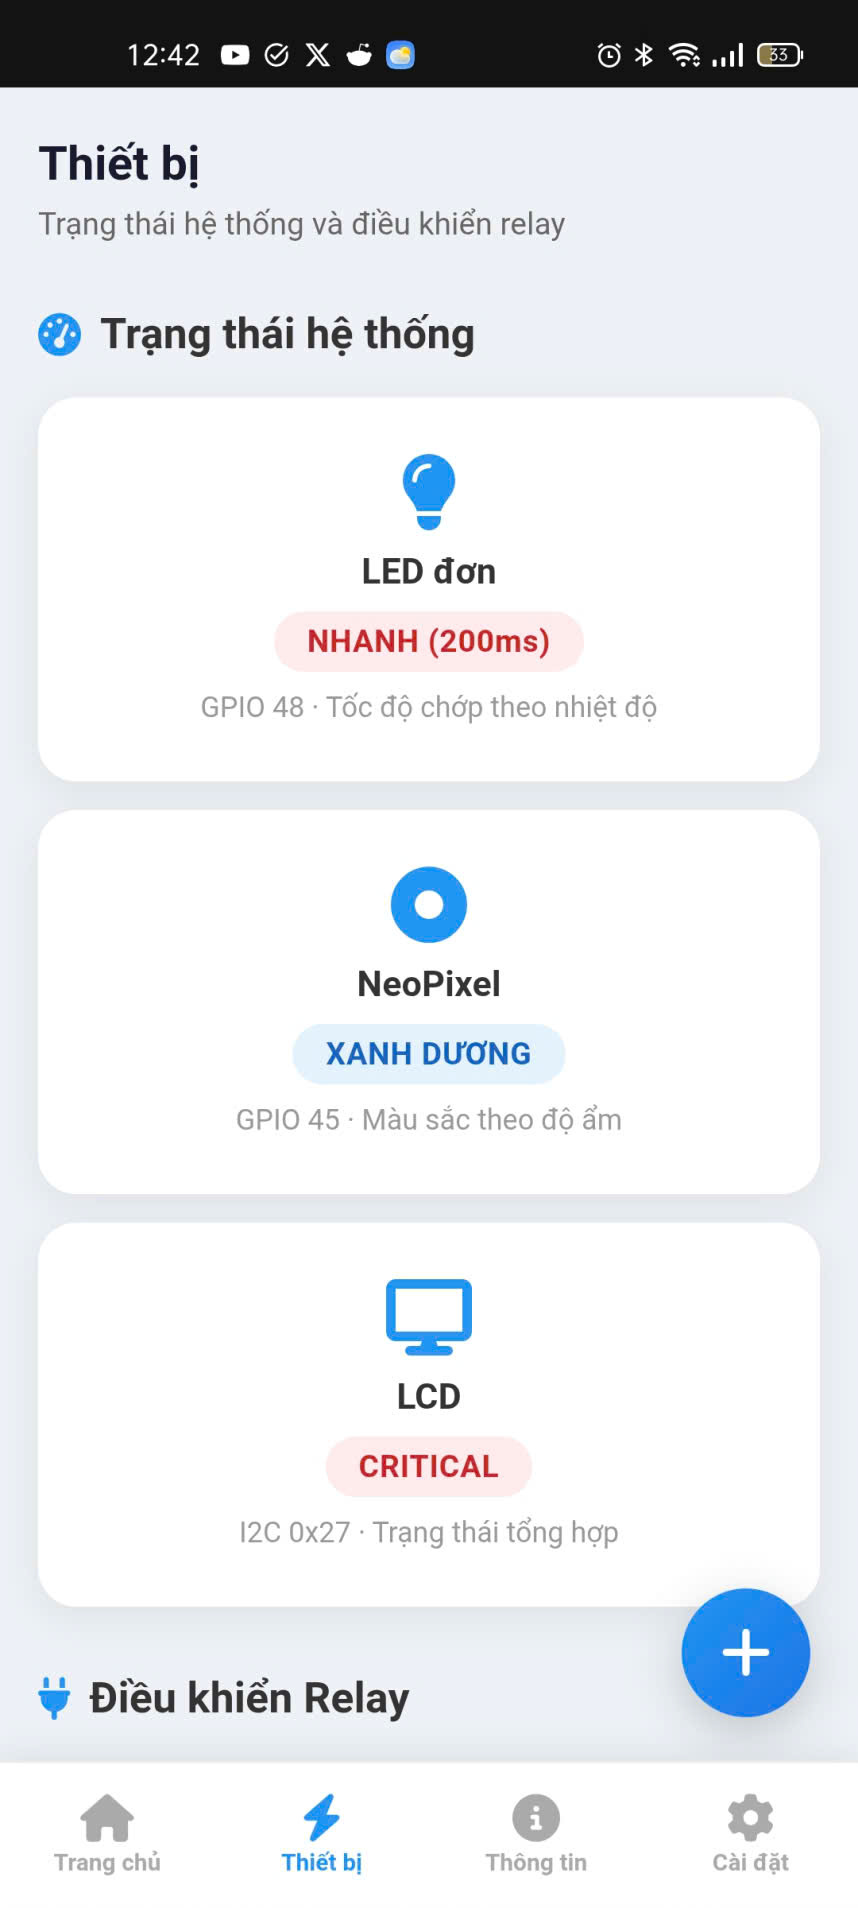
\includegraphics[width=0.9\linewidth, height=0.7\textheight, keepaspectratio]{graphics/peripherals.jpg}
    \caption{Bo mạch YOLO UNO và các thiết bị ngoại vi kết nối}
    \label{fig:peripherals}
\end{figure}

% ============================================================
\section{Kiến Trúc Hệ Thống}
% ============================================================

\subsection{Cấu Trúc Thư Mục}

Mã nguồn được tổ chức theo hướng module hóa, mỗi thư mục con tương ứng một nhóm chức năng:

\begin{itemize}
    \item \texttt{src/actuators/} — Task 1 (LED), Task 2 (NeoPixel)
    \item \texttt{src/sensors/} — Task 3 (DHT20 monitor, LCD task)
    \item \texttt{src/connectivity/} — Quản lý WiFi, LittleFS, nút BOOT
    \item \texttt{src/web\_services/} — Task 4 (AsyncWebServer + WebSocket handler)
    \item \texttt{src/cloud/} — Task 6 (MQTT CoreIOT)
    \item \texttt{src/tinyml/} — Task 5 (TFLite Micro inference, model header, dataset)
    \item \texttt{src/global.cpp} + \texttt{include/global.h} — Khởi tạo và khai báo Queue, Semaphore, struct \texttt{SensorData}
    \item \texttt{data/} — File web tĩnh phục vụ qua LittleFS (HTML, JS, CSS)
\end{itemize}

\subsection{Sơ Đồ Luồng Dữ Liệu}

Toàn bộ dữ liệu cảm biến được phân phối qua hai cơ chế RTOS:

\begin{itemize}
    \item \textbf{xSensorQueue (Mailbox, depth=1):} Task \texttt{temp\_humi\_monitor} ghi struct \texttt{SensorData\{temperature, humidity, lcd\_status\}} vào Queue bằng \texttt{xQueueOverwrite}. Các task LCD, WebServer và TinyML đọc bằng \texttt{xQueuePeek} (không xóa item).
    \item \textbf{9 Binary Semaphore:} 3 semaphore nhiệt độ (Low/Normal/High), 3 semaphore độ ẩm (Low/Normal/High), 3 semaphore trạng thái (Normal/Warning/Critical) — được give theo pattern \textit{edge detection} khi phát hiện thay đổi mức.
\end{itemize}

\subsection{Danh Sách RTOS Tasks}

\begin{table}[H]
\centering
\begin{tabular}{|p{2.8cm}|c|c|p{6.5cm}|}
\hline
\textbf{Task} & \textbf{Stack} & \textbf{Ưu tiên} & \textbf{Vai trò} \\
\hline
LED Blink       & 2048~B & 2 & Điều khiển LED GPIO~48 theo semaphore nhiệt độ \\
NEO Blink       & 2048~B & 2 & Điều khiển NeoPixel GPIO~45 theo semaphore độ ẩm \\
TEMP HUMI       & 4096~B & 2 & Đọc DHT20, gửi Queue + give Semaphore trạng thái \\
LCD Display     & 4096~B & 2 & Nhận Queue, hiển thị LCD 16×2 I2C \\
TinyML          & 4096~B & 2 & TFLite Micro inference, phát hiện bất thường \\
CoreIOT         & 8192~B & 2 & MQTT publish telemetry lên \texttt{app.coreiot.io} \\
WebServer       & 8192~B & 2 & AsyncWebServer + WebSocket real-time dashboard \\
BOOT Toggle     & 4096~B & 2 & Giám sát GPIO~0, xóa LittleFS khi giữ $>$2~s \\
\hline
\end{tabular}
\caption{Danh sách RTOS Task trong hệ thống (hàm tương ứng xem \texttt{src/main.cpp})}
\end{table}


% ============================================================
\section{Kiến Trúc Phần Mềm Của Hệ Thống}
% ============================================================

\subsection{Mô Hình Phân Lớp}

Phần mềm được tổ chức theo 5 lớp từ dưới lên:

\begin{enumerate}
    \item \textbf{Hardware:} ESP32-S3 240~MHz Dual Core.
    \item \textbf{HAL (FreeRTOS + Arduino):} Scheduler, GPIO, I2C, WiFi stack.
    \item \textbf{Connectivity:} \texttt{task\_wifi} (AP+STA), \texttt{task\_check\_info} (LittleFS).
    \item \textbf{Data Bus:} \texttt{xSensorQueue} (Mailbox) + 9 Binary Semaphore.
    \item \textbf{Application:} 8 FreeRTOS Task xử lý nghiệp vụ cụ thể.
\end{enumerate}

\subsection{Quy Trình Khởi Động (Boot Sequence)}

\begin{enumerate}
    \item \texttt{setup()} gọi \texttt{init\_globals()} — tạo toàn bộ Queue và Semaphore \textbf{trước} khi đăng ký bất kỳ task nào.
    \item Lần lượt gọi \texttt{xTaskCreate()} cho 8 task.
    \item FreeRTOS Scheduler bắt đầu điều phối các task.
\end{enumerate}

\textbf{Quy tắc quan trọng:} \texttt{init\_globals()} bắt buộc phải chạy trước \texttt{xTaskCreate()}. Nếu Queue/Semaphore chưa tạo mà task đã gọi \texttt{xSemaphoreTake()}, firmware sẽ crash do NULL pointer dereference.

\subsection{Nguyên Tắc Module Hóa}

\begin{itemize}
    \item \textbf{Single Responsibility:} Mỗi file \texttt{.cpp} chứa đúng 1 FreeRTOS task với 1 chức năng.
    \item \textbf{Không biến toàn cục sensor:} Dữ liệu truyền qua \texttt{xSensorQueue}; trạng thái thiết bị qua Semaphore.
    \item \textbf{Producer-Consumer rõ ràng:} \texttt{temp\_humi\_monitor} là producer duy nhất; các task còn lại là consumer thuần túy.
    \item \textbf{Cấu hình tập trung:} Ngưỡng T/H định nghĩa trong \texttt{include/global.h} — thay đổi một chỗ ảnh hưởng toàn hệ thống.
\end{itemize}


% ============================================================
\section{Các Giải Pháp Triển Khai}
% ============================================================

\subsection{Task 1: LED Blink Theo Nhiệt Độ}

\textbf{Yêu cầu:} LED chớp với 3 tốc độ khác nhau tương ứng ít nhất 3 mức nhiệt độ, sử dụng Semaphore để đồng bộ.

\textbf{Ngưỡng} (định nghĩa trong \texttt{include/global.h}): \texttt{TEMP\_NORMAL\_LOW = 25.0°C}, \texttt{TEMP\_NORMAL\_HIGH = 30.0°C}.

\begin{table}[h!]
\centering
\begin{tabular}{|l|l|c|}
\hline
\textbf{Mức nhiệt độ} & \textbf{Semaphore} & \textbf{Khoảng chớp} \\
\hline
Lạnh: $T < 25°C$ & \texttt{xTempLowSemaphore} & 2000~ms \\
Bình thường: $25 \leq T \leq 30°C$ & \texttt{xTempNormalSemaphore} & 1000~ms \\
Nóng: $T > 30°C$ & \texttt{xTempHighSemaphore} & 200~ms \\
\hline
\end{tabular}
\caption{Ánh xạ mức nhiệt độ sang tốc độ LED}
\end{table}

\textbf{Giải pháp — Edge Detection Semaphore:} Task \texttt{temp\_humi\_monitor} theo dõi biến \texttt{last\_temp} và chỉ \texttt{xSemaphoreGive} khi phát hiện thay đổi mức, không give ở mỗi chu kỳ đọc. Task \texttt{led\_blinky} poll 3 semaphore với timeout = 0 (non-blocking) và duy trì \texttt{blinkInterval} cho đến khi có semaphore mới.

\subsection{Task 2: NeoPixel RGB Theo Độ Ẩm}

\textbf{Yêu cầu:} NeoPixel hiển thị 3 màu tương ứng 3 mức độ ẩm.

\textbf{Ngưỡng:} \texttt{HUMI\_NORMAL\_LOW = 40.0\%}, \texttt{HUMI\_NORMAL\_HIGH = 60.0\%}.

\begin{table}[h!]
\centering
\begin{tabular}{|l|l|l|l|}
\hline
\textbf{Mức độ ẩm} & \textbf{Semaphore} & \textbf{Màu} & \textbf{RGB} \\
\hline
Khô: $H < 40\%$ & \texttt{xHumiLowSemaphore} & Đỏ & (255, 0, 0) \\
Bình thường: $40 \leq H \leq 60\%$ & \texttt{xHumiNormalSemaphore} & Xanh lá & (0, 255, 0) \\
Ẩm: $H > 60\%$ & \texttt{xHumiHighSemaphore} & Xanh dương & (0, 0, 255) \\
\hline
\end{tabular}
\caption{Ánh xạ mức độ ẩm sang màu NeoPixel}
\end{table}

Cơ chế edge detection và poll semaphore tương tự Task~1. NeoPixel khởi tạo với độ sáng 50\% bằng \texttt{pixels.setBrightness(50)}, thư viện \texttt{Adafruit\_NeoPixel}.

\subsection{Task 3: LCD và Loại Bỏ Biến Toàn Cục}

\textbf{Yêu cầu:} Hiển thị 3 trạng thái trên LCD, loại bỏ \textbf{hoàn toàn} biến toàn cục liên quan đến cảm biến.

\subsubsection{Struct SensorData Thay Thế Biến Toàn Cục}

Thay vì dùng \texttt{float glob\_temp; float glob\_humi;}, toàn bộ dữ liệu sensor được đóng gói trong struct duy nhất:

\begin{lstlisting}[language=C++, caption=Struct SensorData trong include/global.h]
struct SensorData {
    float temperature;
    float humidity;
    int   lcd_status;  // 0=NORMAL, 1=WARNING, 2=CRITICAL
};
\end{lstlisting}

\subsubsection{Mailbox Queue}

Queue được tạo với depth = 1 (mailbox pattern). Producer dùng \texttt{xQueueOverwrite} (không block), consumer dùng \texttt{xQueuePeek} (không xóa item):

\begin{itemize}
    \item LCD, WebServer và TinyML cùng đọc một item — không task nào "ăn mất" dữ liệu của task khác.
    \item Producer không bao giờ bị block khi queue đầy.
\end{itemize}

\subsubsection{Logic Trạng Thái LCD}

\begin{itemize}
    \item \textbf{CRITICAL (2):} $T > 30°C$
    \item \textbf{WARNING (1):} $T \geq 25°C$ hoặc $H < 40\%$ hoặc $H > 60\%$
    \item \textbf{NORMAL (0):} Tất cả điều kiện còn lại
\end{itemize}

\subsection{Task 4: Web Server AP Mode}

\textbf{Yêu cầu:} Web server hoạt động ở chế độ AP, điều khiển ít nhất 2 thiết bị, giao diện có ít nhất 2 nút.

\subsubsection{Kiến Trúc WebSocket}

Sử dụng \textbf{ESPAsyncWebServer} + \textbf{AsyncWebSocket} thay vì HTTP polling, cho phép cập nhật dữ liệu thời gian thực không cần tải lại trang. Endpoint: \texttt{/ws}, HTTP port 80, file tĩnh từ LittleFS.

\subsubsection{Chế Độ WiFi AP+STA Đồng Thời}

\begin{lstlisting}[language=C++, caption=Cấu hình WIFI\_AP\_STA trong task\_wifi.cpp]
WiFi.mode(WIFI_AP_STA);
WiFi.softAP("ESP32 LOCAL", "12345678");  // IP: 192.168.4.1
\end{lstlisting}

Đảm bảo dashboard luôn truy cập được qua IP \texttt{192.168.4.1} ngay cả khi chưa có kết nối Internet.

\subsubsection{Dashboard 4 Trang}

\begin{enumerate}
    \item \textbf{Home:} Hai đồng hồ gauge (JustGage + Raphael.js) hiển thị T/H thời gian thực.
    \item \textbf{Device:} Trạng thái LED, NeoPixel, LCD và điều khiển relay động (thêm/xóa relay qua GPIO).
    \item \textbf{Info:} Địa chỉ IP, uptime, cấu hình AP/STA, thông tin CoreIOT.
    \item \textbf{Settings:} Form cấu hình WiFi (có nút quét mạng) và CoreIOT token; sau khi lưu thiết bị tự khởi động lại.
\end{enumerate}

\begin{figure}[H]
    \centering
    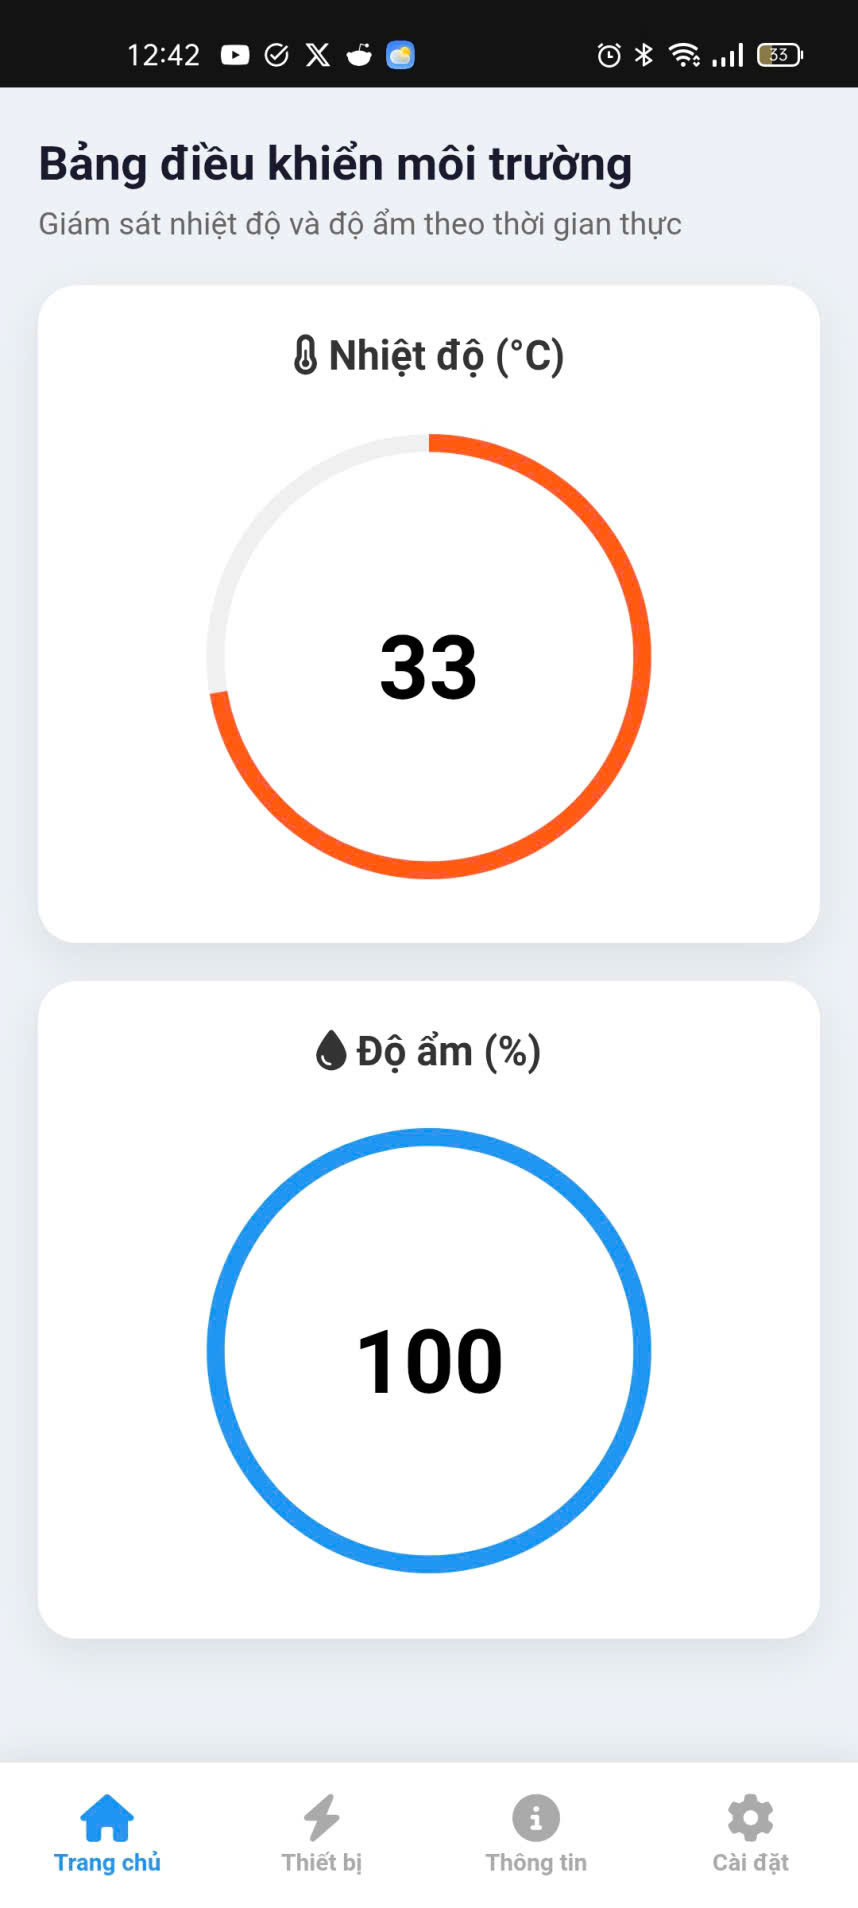
\includegraphics[width=0.9\linewidth, height=0.7\textheight, keepaspectratio]{graphics/temp-humid-dashboard.jpg}
    \caption{Dashboard — Trang Home: gauge nhiệt độ \& độ ẩm thời gian thực}
    \label{fig:dashboard-home}
\end{figure}

\begin{figure}[H]
    \centering
    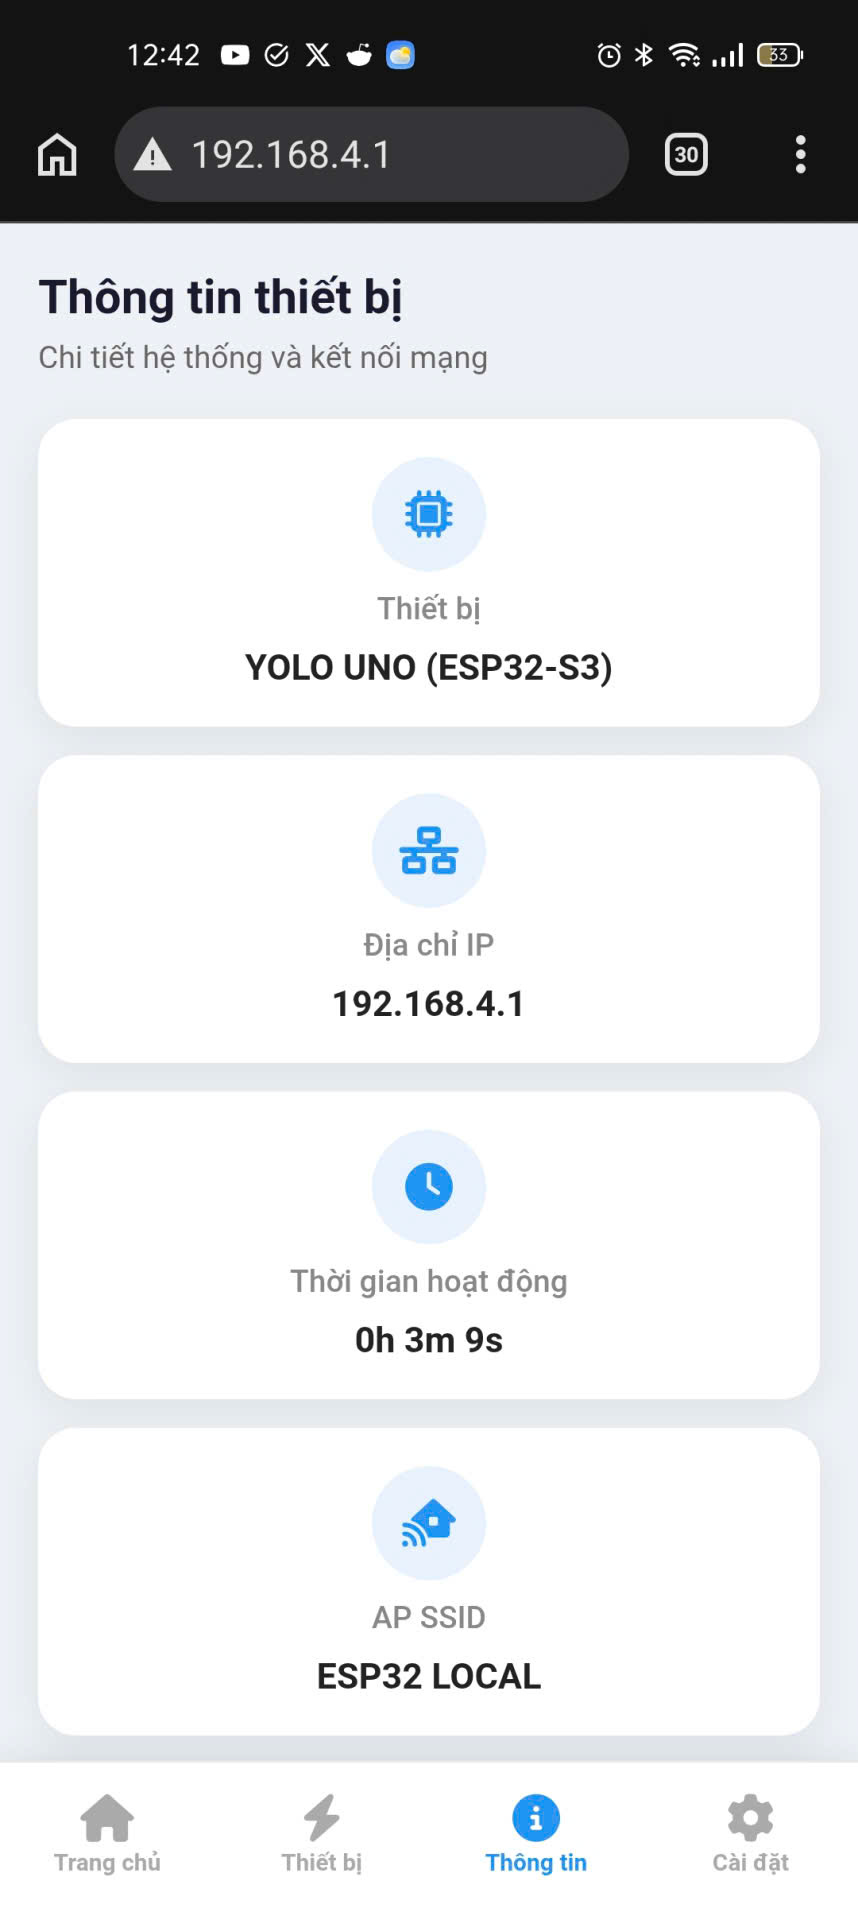
\includegraphics[width=0.9\linewidth, height=0.7\textheight, keepaspectratio]{graphics/devices.jpg}
    \caption{Dashboard — Trang Device: điều khiển relay động qua WebSocket}
    \label{fig:dashboard-device}
\end{figure}

\begin{figure}[H]
    \centering
    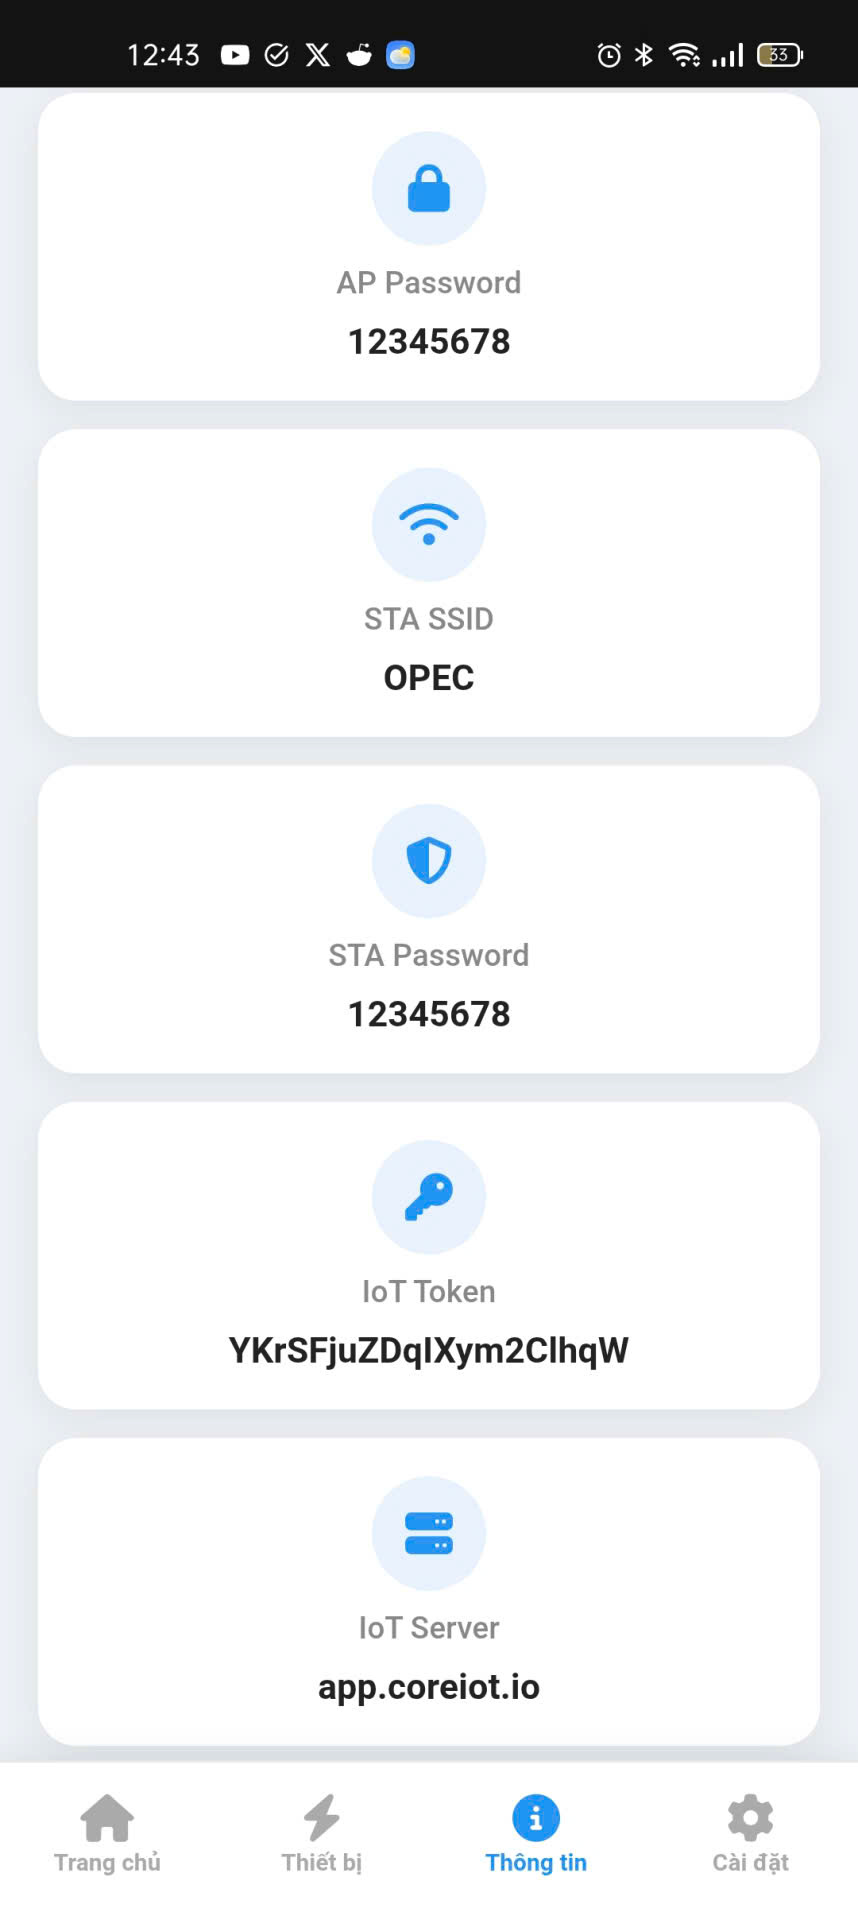
\includegraphics[width=0.9\linewidth, height=0.7\textheight, keepaspectratio]{graphics/connectivity.jpg}
    \caption{Dashboard — Trang Info: thông tin kết nối WiFi AP/STA}
    \label{fig:dashboard-info}
\end{figure}

\begin{figure}[H]
    \centering
    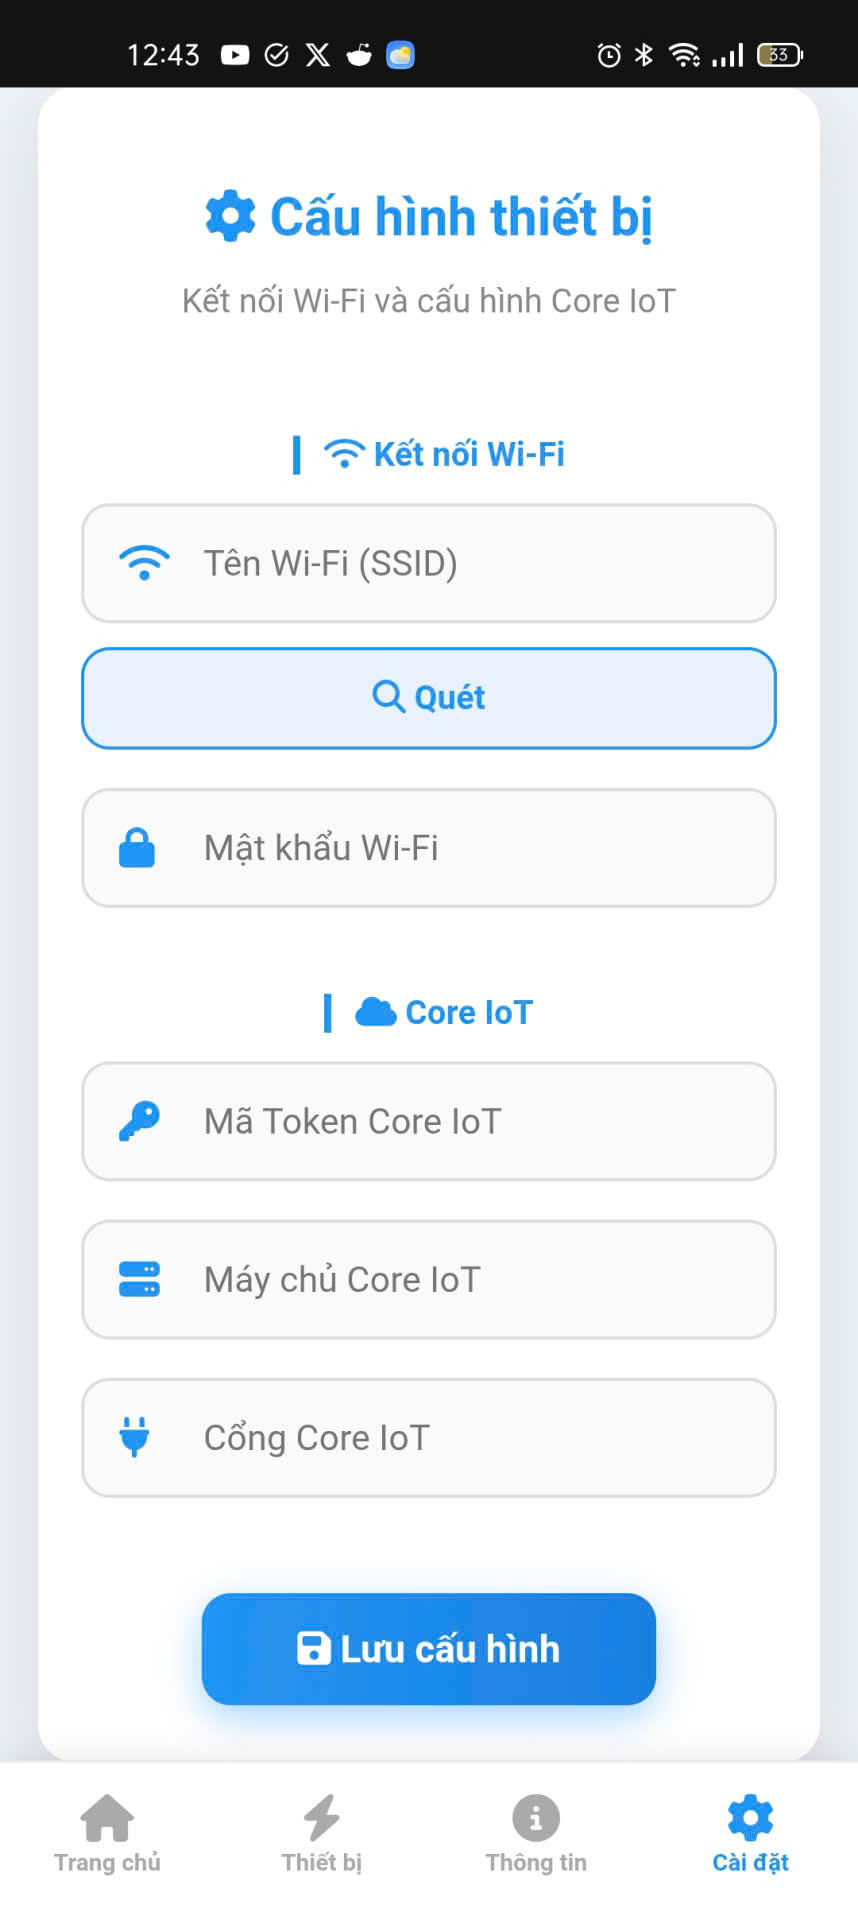
\includegraphics[width=0.9\linewidth, height=0.7\textheight, keepaspectratio]{graphics/configs.jpg}
    \caption{Dashboard — Trang Settings: cấu hình WiFi \& CoreIOT token}
    \label{fig:dashboard-settings}
\end{figure}

\subsection{Task 5: TinyML — Phát Hiện Bất Thường}

\textbf{Yêu cầu:} Triển khai mô hình TinyML trên vi điều khiển, mô tả dataset, đánh giá độ chính xác.

\subsubsection{Dataset}

2000 mẫu tổng hợp (\texttt{custom\_iot\_dataset.csv}):
\begin{itemize}
    \item \textbf{Normal (80\%):} $25 \leq T \leq 30°C$ và $40 \leq H \leq 60\%$
    \item \textbf{Anomaly (20\%):} Nóng ($T>35°C$), Lạnh ($T<20°C$), Ẩm ($H>70\%$), Khô ($H<30\%$)
\end{itemize}

\subsubsection{Kiến Trúc Mô Hình ANN}

\[
\text{Input}(2) \rightarrow \text{Dense}(8, \text{ReLU}) \rightarrow \text{Dense}(1, \text{Sigmoid})
\]

Tổng 33 tham số, kích thước \texttt{.tflite}: \textbf{1928 bytes}. Tensor arena: 10~KB.

\subsubsection{Tiền Xử Lý Z-score}

Hằng số chuẩn hóa nhúng trực tiếp vào firmware:
\begin{lstlisting}[language=C++, caption=Hằng số Z-score trong tinyml.cpp]
const float SCALER_MEAN[]  = {27.4874f, 49.9192f};
const float SCALER_SCALE[] = {4.2157f,  12.0575f};
\end{lstlisting}

\subsubsection{Kết Quả Đánh Giá}

\begin{itemize}
    \item Train accuracy: \textbf{99.44\%} (epoch 100)
    \item 6/6 test case biên (nóng, lạnh, ẩm, khô, sát biên) cho kết quả đúng.
    \item Hạn chế: Dataset tổng hợp, chưa đánh giá trên dữ liệu thực tế từ cảm biến.
\end{itemize}

\subsection{Task 6: CoreIOT Cloud (MQTT)}

\textbf{Yêu cầu:} Đẩy sensor data lên CoreIOT, ESP32-S3 ở chế độ STA, dùng đúng access token.

\subsubsection{Cấu Hình MQTT}

\begin{itemize}
    \item Thư viện: \textbf{PubSubClient}
    \item Server: \texttt{app.coreiot.io}, port \texttt{1883}
    \item Topic: \texttt{esp/telemetry}
    \item Xác thực ThingsBoard: username = access token, password = rỗng
    \item ClientID: \texttt{"ESP32\_" + WiFi.macAddress()} (đảm bảo tính duy nhất)
\end{itemize}

\subsubsection{Đồng Bộ Với WiFi}

Task \texttt{task\_core\_iot} chờ semaphore \texttt{xBinarySemaphoreInternet} — được give trong WiFi event callback \texttt{ARDUINO\_EVENT\_WIFI\_STA\_GOT\_IP} khi STA nhận được IP. Đảm bảo không cố kết nối MQTT trước khi có Internet.

\subsubsection{Payload Telemetry}

Mỗi 10 giây, task đọc \texttt{xSensorQueue} và publish JSON:
\begin{lstlisting}[language=JSON, caption=Cấu trúc payload gửi lên CoreIOT]
{"temperature": 28.5, "humidity": 55.3}
\end{lstlisting}

\begin{figure}[H]
    \centering
    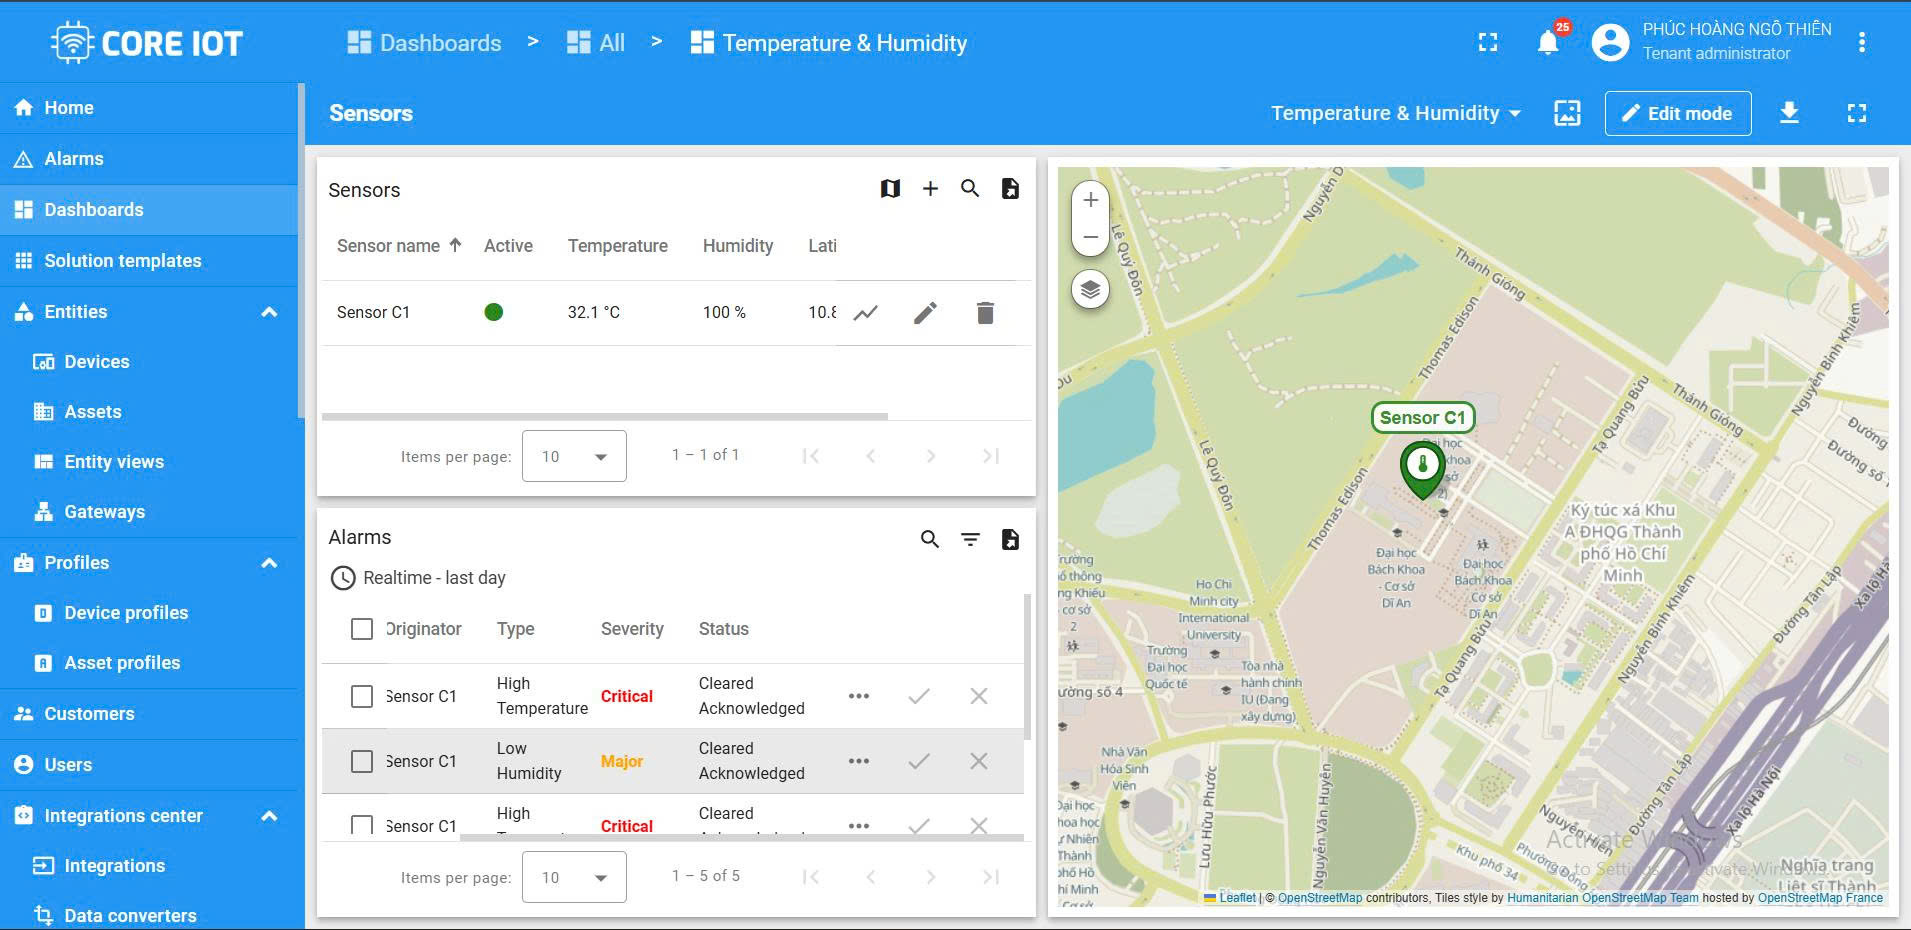
\includegraphics[width=0.9\linewidth, height=0.7\textheight, keepaspectratio]{graphics/coreiot-dashboard.jpg}
    \caption{Dashboard CoreIOT nhận telemetry nhiệt độ và độ ẩm từ ESP32-S3 \cite{coreiot}}
    \label{fig:coreiot}
\end{figure}

% ============================================================
\section{Cơ Chế Đồng Bộ (Semaphore \& Queue)}
% ============================================================

\subsection{Tổng Quan Các Đối Tượng RTOS}

Tất cả Queue và Semaphore khai báo trong \texttt{include/global.h}, khởi tạo trong \texttt{src/global.cpp} hàm \texttt{init\_globals()}.

\begin{table}[H]
\centering
\begin{tabular}{|l|l|l|p{5cm}|}
\hline
\textbf{Tên} & \textbf{Loại} & \textbf{Depth} & \textbf{Mục đích} \\
\hline
\texttt{xSensorQueue} & Queue & 1 (Mailbox) & Truyền \texttt{SensorData} từ monitor sang LCD/WebServer/TinyML \\
\hline
\end{tabular}
\caption{Queue trong hệ thống}
\end{table}

\begin{table}[H]
\centering
\begin{tabular}{|l|l|l|}
\hline
\textbf{Semaphore} & \textbf{Give bởi} & \textbf{Take bởi} \\
\hline
\texttt{xTempLowSemaphore} & \texttt{temp\_humi\_monitor} & \texttt{led\_blinky} \\
\texttt{xTempNormalSemaphore} & \texttt{temp\_humi\_monitor} & \texttt{led\_blinky} \\
\texttt{xTempHighSemaphore} & \texttt{temp\_humi\_monitor} & \texttt{led\_blinky} \\
\texttt{xHumiLowSemaphore} & \texttt{temp\_humi\_monitor} & \texttt{neo\_blinky} \\
\texttt{xHumiNormalSemaphore} & \texttt{temp\_humi\_monitor} & \texttt{neo\_blinky} \\
\texttt{xHumiHighSemaphore} & \texttt{temp\_humi\_monitor} & \texttt{neo\_blinky} \\
\texttt{xStatusNormalSemaphore} & monitor + tiny\_ml & \texttt{lcd\_task} \\
\texttt{xStatusWarningSemaphore} & monitor + tiny\_ml & \texttt{lcd\_task} \\
\texttt{xStatusCriticalSemaphore} & \texttt{temp\_humi\_monitor} & \texttt{lcd\_task} \\
\texttt{xBinarySemaphoreInternet} & WiFi event callback & \texttt{task\_core\_iot} \\
\hline
\end{tabular}
\caption{Danh sách 9 Binary Semaphore và 1 Internet Semaphore}
\end{table}

\subsection{Pattern: Edge Detection}

Producer chỉ give semaphore khi \textbf{phát hiện thay đổi mức} (không give ở mỗi chu kỳ đọc). Consumer dùng \texttt{xSemaphoreTake(..., 0)} (non-blocking poll) và duy trì state cuối cùng. Tránh semaphore bị "cộng dồn" và giảm tải FreeRTOS scheduler.

\subsection{Pattern: Mailbox Queue với Overwrite}

\texttt{xSensorQueue} (depth=1) hoạt động như mailbox:
\begin{itemize}
    \item Producer: \texttt{xQueueOverwrite} — ghi đè giá trị cũ, không bao giờ block.
    \item Consumer: \texttt{xQueuePeek} — đọc không xóa, nhiều task đọc cùng lúc an toàn.
\end{itemize}


% ============================================================
\section{Kết Quả \& Đánh Giá}
% ============================================================

\subsection{Task 1 — LED Blink}
\textbf{Hoàn thành.} LED GPIO~48 chớp đúng 3 tốc độ. Semaphore edge detection hoạt động chính xác.

\subsection{Task 2 — NeoPixel}
\textbf{Hoàn thành.} NeoPixel GPIO~45 hiển thị 3 màu theo độ ẩm. Màu cập nhật ngay khi semaphore được give.

\subsection{Task 3 — LCD \& Loại Bỏ Biến Toàn Cục}
\textbf{Hoàn thành.} Không có biến toàn cục \texttt{float} nào liên quan đến sensor. \texttt{xQueuePeek} cho phép WebServer và TinyML cùng đọc dữ liệu không xung đột. LCD cập nhật 500~ms/lần với 3 trạng thái.

\subsection{Task 4 — Web Server}
\textbf{Hoàn thành chức năng cốt lõi.} Dashboard 4 trang, gauge thời gian thực, điều khiển relay động, quét WiFi, cấu hình CoreIOT. \textit{Điểm cần cải tiến:} danh sách relay chưa được lưu vào LittleFS, mất sau khi tải lại trang.

\subsection{Task 5 — TinyML}
\textbf{Đã triển khai, cần đánh giá thực tế.} Mô hình ANN 1928~bytes chạy trên ESP32-S3, tensor arena 10~KB. 99.44\% accuracy trên dataset tổng hợp \cite{kaggle-iot-anomaly}, 6/6 test case biên đúng. Chưa có đánh giá trên dữ liệu thực từ phần cứng.

\begin{figure}[H]
    \centering
    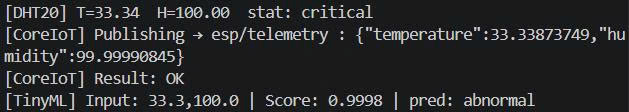
\includegraphics[width=0.9\linewidth, height=0.7\textheight, keepaspectratio]{graphics/serial-log.jpg}
    \caption{Serial Monitor hiển thị kết quả inference TinyML trên ESP32-S3}
    \label{fig:serial-log}
\end{figure}

\subsection{Task 6 — CoreIOT Cloud}
\textbf{Code hoàn chỉnh, cần cấu hình token.} Logic MQTT đầy đủ (kết nối, xác thực ThingsBoard, publish JSON, reconnect). Cần nhập access token thực tế qua trang Settings của dashboard.


% ============================================================
\section{Mã Nguồn — Các Đoạn Code Quan Trọng}
% ============================================================

\subsection{Khởi Tạo Hệ Thống}

\begin{lstlisting}[language=C++, caption=init\_globals() trong src/global.cpp]
void init_globals() {
    xSensorQueue = xQueueCreate(1, sizeof(struct SensorData));
    xTempLowSemaphore    = xSemaphoreCreateBinary();
    xTempNormalSemaphore = xSemaphoreCreateBinary();
    xTempHighSemaphore   = xSemaphoreCreateBinary();
    xHumiLowSemaphore    = xSemaphoreCreateBinary();
    xHumiNormalSemaphore = xSemaphoreCreateBinary();
    xHumiHighSemaphore   = xSemaphoreCreateBinary();
    xStatusNormalSemaphore   = xSemaphoreCreateBinary();
    xStatusWarningSemaphore  = xSemaphoreCreateBinary();
    xStatusCriticalSemaphore = xSemaphoreCreateBinary();
    xBinarySemaphoreInternet = xSemaphoreCreateBinary();
    xSemaphoreGive(xStatusNormalSemaphore); // Khoi dong o Normal
}
\end{lstlisting}

\subsection{Edge Detection Semaphore (Task 1)}

\begin{lstlisting}[language=C++, caption=Producer - edge detection trong temp\_humi\_monitor.cpp]
if (temperature < TEMP_NORMAL_LOW && last_temp >= TEMP_NORMAL_LOW) {
    xSemaphoreGive(xTempLowSemaphore);
} else if (temperature >= TEMP_NORMAL_LOW && temperature <= TEMP_NORMAL_HIGH
           && (last_temp < TEMP_NORMAL_LOW || last_temp > TEMP_NORMAL_HIGH)) {
    xSemaphoreGive(xTempNormalSemaphore);
} else if (temperature > TEMP_NORMAL_HIGH && last_temp <= TEMP_NORMAL_HIGH) {
    xSemaphoreGive(xTempHighSemaphore);
}
last_temp = temperature;
\end{lstlisting}

\begin{lstlisting}[language=C++, caption=Consumer - non-blocking poll trong led\_blinky.cpp]
if      (xSemaphoreTake(xTempHighSemaphore,   0) == pdTRUE) blinkInterval = 200;
else if (xSemaphoreTake(xTempNormalSemaphore, 0) == pdTRUE) blinkInterval = 1000;
else if (xSemaphoreTake(xTempLowSemaphore,    0) == pdTRUE) blinkInterval = 2000;
\end{lstlisting}

\subsection{Mailbox Queue (Task 3)}

\begin{lstlisting}[language=C++, caption=Producer dung xQueueOverwrite - temp\_humi\_monitor.cpp]
struct SensorData data = {temperature, humidity, lcd_status};
xQueueOverwrite(xSensorQueue, &data);
\end{lstlisting}

\begin{lstlisting}[language=C++, caption=Consumer dung xQueuePeek - lcd\_task.cpp]
struct SensorData currentData;
xQueuePeek(xSensorQueue, &currentData, pdMS_TO_TICKS(100));
\end{lstlisting}

\subsection{TFLite Micro Inference (Task 5)}

\begin{lstlisting}[language=C++, caption=Z-score va inference trong tinyml.cpp]
input->data.f[0] = (sensorData.temperature - SCALER_MEAN[0]) / SCALER_SCALE[0];
input->data.f[1] = (sensorData.humidity    - SCALER_MEAN[1]) / SCALER_SCALE[1];
interpreter->Invoke();
float score = output->data.f[0];
if (score > 0.5f) xSemaphoreGive(xStatusWarningSemaphore);
else              xSemaphoreGive(xStatusNormalSemaphore);
\end{lstlisting}

\subsection{MQTT CoreIOT (Task 6)}

\begin{lstlisting}[language=C++, caption=Publish telemetry trong task\_core\_iot.cpp]
xSemaphoreTake(xBinarySemaphoreInternet, pdMS_TO_TICKS(5000));
xSemaphoreGive(xBinarySemaphoreInternet);  // Tra lai cho task khac

mqttClient.connect(clientId.c_str(), ACCESS_TOKEN, "");

char payload[64];
snprintf(payload, sizeof(payload),
         "{\"temperature\":%.2f,\"humidity\":%.2f}",
         data.temperature, data.humidity);
mqttClient.publish("esp/telemetry", payload);
\end{lstlisting}


% ============================================================
\section{Kết Luận}
% ============================================================

\subsection{Tóm Tắt Thành Tựu}

\begin{itemize}
    \item \textbf{Task 1, 2, 3:} Hoàn thành đầy đủ — semaphore, queue, loại bỏ biến toàn cục.
    \item \textbf{Task 4:} Hoàn thành chức năng cốt lõi — WebSocket dashboard đa trang, relay động.
    \item \textbf{Task 5:} Đã triển khai — TinyML ANN 99.44\% accuracy trên ESP32-S3.
    \item \textbf{Task 6:} Code hoàn chỉnh — chờ cấu hình token thực tế.
\end{itemize}

\subsection{Điểm Cần Cải Thiện}

\begin{enumerate}
    \item \textbf{Task 4:} Lưu cấu hình relay vào LittleFS để không mất sau khởi động lại.
    \item \textbf{Task 5:} Thu thập dataset thực tế từ cảm biến và đánh giá accuracy trên phần cứng.
    \item \textbf{Task 6:} Cấu hình token thực và kiểm tra truyền dữ liệu end-to-end lên CoreIOT.
\end{enumerate}

\subsection{Bài Học Kinh Nghiệm}

\begin{itemize}
    \item \textbf{Mailbox pattern} (\texttt{xQueueCreate(1)} + \texttt{xQueueOverwrite} + \texttt{xQueuePeek}): tối ưu cho dữ liệu "chỉ cần giá trị mới nhất", không block producer, không cạnh tranh giữa các consumer.
    \item \textbf{Edge detection semaphore}: tốt hơn level detection vì tránh tràn binary semaphore và giảm tải scheduler.
    \item \textbf{WiFi AP+STA đồng thời}: giải quyết mâu thuẫn giữa Task~4 (cần AP) và Task~6 (cần STA).
    \item \textbf{TFLite Micro}: yêu cầu định dạng \texttt{.tflite} flatbuffer từ TensorFlow/Keras; kích thước tensor arena cần điều chỉnh theo kiến trúc model.
    \item \textbf{Init trước task creation}: \texttt{init\_globals()} phải gọi trong \texttt{setup()} trước \texttt{xTaskCreate()} để tránh race condition.
\end{itemize}

% ============================================================
\section*{Mã Nguồn}
\addcontentsline{toc}{section}{Mã Nguồn}
% ============================================================

Toàn bộ mã nguồn của dự án được lưu trữ công khai trên GitHub:

\begin{center}
    \url{https://github.com/thienphucope/iot252}
\end{center}

Repository bao gồm mã nguồn PlatformIO (C++), notebook huấn luyện TinyML (Python/Jupyter), dataset tổng hợp và tài liệu kỹ thuật.

% ============================================================
\section*{Tài Liệu Tham Khảo}
\addcontentsline{toc}{section}{Tài Liệu Tham Khảo}
% ============================================================

\begin{thebibliography}{99}

\bibitem{freertos}
Real Time Engineers Ltd.,
\textit{FreeRTOS — Real-time operating system for microcontrollers},
\url{https://www.freertos.org}, truy cập 2026.

\bibitem{esp32s3}
Espressif Systems,
\textit{ESP32-S3 Technical Reference Manual},
Espressif Systems, 2022.
\url{https://www.espressif.com/sites/default/files/documentation/esp32-s3_technical_reference_manual_en.pdf}

\bibitem{tflite-micro}
TensorFlow Authors,
\textit{TensorFlow Lite for Microcontrollers},
\url{https://www.tensorflow.org/lite/microcontrollers}, truy cập 2026.

\bibitem{kaggle-iot-anomaly}
S. (smmmmmmmmmmmm),
\textit{Anomaly Detection in IoT Devices — Synthetic Dataset (2000 samples)},
Kaggle, 2024.
\url{https://www.kaggle.com/datasets/smmmmmmmmmmmm/anomaly-detection-in-iot-devices}

\bibitem{coreiot}
CoreIOT Platform (ThingsBoard-based),
\textit{CoreIOT Cloud Dashboard},
\url{https://app.coreiot.io}, truy cập 2026.

\bibitem{espassync}
M. Hightower et al.,
\textit{ESPAsyncWebServer — Async HTTP and WebSocket Server for ESP32},
GitHub, 2021.
\url{https://github.com/me-no-dev/ESPAsyncWebServer}

\bibitem{pubsubclient}
N. O'Leary,
\textit{PubSubClient — MQTT Client for Arduino},
\url{https://pubsubclient.knolleary.net}, truy cập 2026.

\bibitem{adafruit-neo}
Adafruit Industries,
\textit{Adafruit NeoPixel Library for Arduino},
GitHub, 2023.
\url{https://github.com/adafruit/Adafruit_NeoPixel}

\bibitem{platformio}
PlatformIO Labs,
\textit{PlatformIO — Professional collaborative platform for embedded development},
\url{https://platformio.org}, truy cập 2026.

\bibitem{sourcecode}
Nhóm sinh viên,
\textit{Mã nguồn dự án: YoloUNO PlatformIO-RTOS},
GitHub, 2026.
\url{https://github.com/thienphucope/iot252}

\end{thebibliography}

\end{document}
